\section{Distillation collumn control}
\subsection{Description}
The various control strategies and problems (such as inferential composition measurement) associated with distillation column control can be investigated on the rig shown in figure~\ref{fig:rig:dist}. \begin{figure}
	\centering
	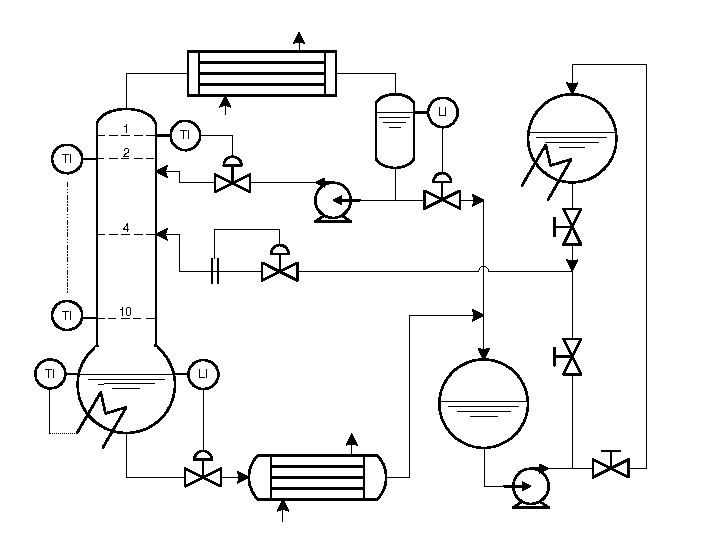
\includegraphics{Dist}
	\caption{The distillation control loop}
	\label{fig:rig:dist}
\end{figure}
Strategies that can be implemented include:
\begin{itemize}
	\item Base layer control system development
	\item Decoupling design and implementation
	\item Constrained model predictive control
	\item Temperature or composition profile control
	\item Non-linear control
	\item Automated start-up and shut down 
\end{itemize}

There are certain control problems unique to this experimental rig. The boiler-accumulator at the bottom of the distillation column is spherical. This makes the level control as well as the boil-up rate highly non-linear. Another control problem identified is that the product is mixed and recycled to the feed drum. This results in output variance being recycled back into the column.

\subsection{Procedures}
\subsubsection{Start-up}
\begin{enumerate}
	\item Open the air supply line.
	\item Adjust the pressure regulator to deliver 200 kPa.
	\item Open \tagname{05HV001} by 10\% (Small fraction).
	\item Set \tagname{05CV002} (feed valve) to 100\%.
	\item Close \tagname{05CV002} when \tagname{05LC001} (Bottoms level) is 80\%.
	\item Switch \tagname{05HS001} (thyristor power) on.
	\item Press the ``Start'' button on the thyristor.
	\item Open the cooling water supply.
	\item Set \tagname{05VC001} (thyristor) to 100\%.
	\item Set \tagname{05VC001} to desired set point when \tagname{05TI001} is more than 60 \deg C.
	\item Switch \tagname{05HS002} on (Reflux pump) when \tagname{05LC002} (Distillate level) is 50\%.
	\item Open \tagname{05CV003} (Reflux) to desired set point.
	\item Set \tagname{05CV002} to the desired set point when \tagname{05TI001} and \tagname{05TI010} stabilises.
	\item Set \tagname{05CV004} (Top) to desired set point.
	\item Set \tagname{05CV005} (Bottom) to desired set point.
\end{enumerate}

\subsubsection{Shut down}
\begin{enumerate}
	\item Close \tagname{05CV002} (Feed)
	\item Close \tagname{05CV004} (Top)
	\item Close \tagname{05CV005} (Bottom)
	\item Switch \tagname{05HS002} off (Reflux pump)
	\item Close \tagname{05CV003} (Reflux valve)
	\item Set \tagname{05VC001} (Thyristor) to 0\%
	\item Switch \tagname{05HS001} off (Thyristor power)
	\item Close the air supply line
	\item Close \tagname{05HV001} when the air pressure is zero
	\item Close the cooling water when \tagname{05TI001} is less than 60 \deg C
\end{enumerate}
